\documentclass[12pt]{article}
\usepackage{graphicx}
\usepackage{hyperref}

\usepackage{tikz}
\usepackage[default]{lato}
\usepackage[T1]{fontenc}
\usepackage{titlesec}
\usepackage{titling}
\usepackage[hmargin=0.5in,bmargin=1in,tmargin=1in,centering]{geometry}
\usetikzlibrary{shadows.blur}
\usetikzlibrary{shapes.symbols}
\usetikzlibrary{positioning,fit,hobby}

% The red used throughout the document
\definecolor{red}{HTML}{D32D2D}
\pagenumbering{gobble}  

% Defines the red lines at the top and bottom of each page
\newcommand\AddLines{%
\begin{tikzpicture}[remember picture,overlay]
    \fill[red] (current page.north west) rectangle ([yshift=-2mm]current page.north east);
    \fill[red] (current page.south west) rectangle ([yshift=2mm]current page.south east);
    \end{tikzpicture}%
}

% Adds the red lines to each page
\AtBeginShipout{\AddLines}
\AtBeginShipoutFirst{\AddLines}

% Defines the red block for section titles
\newcommand\SecTitle[1]{%
\begin{tikzpicture}
  \node[inner ysep=1cm,text width=\paperwidth,fill=red,text=white,font=\Huge]  at (0,0) 
 {\parbox{0.4in}{\mbox{}}\parbox{\dimexpr\textwidth-0.4in\relax}{\raggedright\strut#1\strut}\parbox{0pt}{\mbox{}}};
\end{tikzpicture}%
}

% Adds the red block to section titles
\titleformat{\section}{\normalfont}{}{-0.5in}{\SecTitle}

% NO MORE INDENTS
\setlength\parindent{0pt}
\title{IOT Homecare}

\begin{document}
    \newcommand{\titleimage}{iot.png}
    \newcommand{\titlecompany}{Epi-Use}
    \tikzstyle{title}=[font=\fontsize{32}{144}\selectfont]
\tikzstyle{date}=[font=\fontsize{30}{144}\selectfont]
\tikzstyle{subtitle}=[font=\fontsize{20}{144}\selectfont, white]
\begin{titlepage}        
        \begin{tikzpicture}[remember picture,overlay, anchor = west]
            % Graphic
            \node at (-1.5,-16) {\includegraphics[width=\paperwidth]{\titleimage}};
            
            % Header
            \fill[red] (current page.north west) rectangle ([yshift=-8cm]current page.north east);
            \node[title] (title) at (-0.5,0) {\thetitle};
            \draw[line width=0.75mm, white] ([yshift=-1cm]title.west) -- ([yshift=-1cm]title.east);
            \node[subtitle] at ([yshift=-1.6cm, xshift=-2.4cm]title.east) {Tender};
            
            % Logos
            \node at (-0.8,-22.5)
            {
\includegraphics[width=4cm]{../Common/UniversityOfPretoriaLogo.png}};
            \node at (15,-23.3) {
\includegraphics[width=5cm]{../Common/AlbertPrimeLogo.png}};  
            
            % Hexagon
            \draw[line width=1mm, white] (14.4,-5.1) -- (14.4,-4) -- (16.4,-2.75) -- (18.4,-4) -- (18.4,-5.1);
            \node[date, white] at (15.05,-4.5) {May};
            \draw[line width=1mm, red] (14.4,-5.1) -- (14.4,-6.35) -- (16.4,-7.6) -- (18.4,-6.35) -- (18.4,-5.1);
            \node[date, red] at (15.1,-6) {2017};
            
        \end{tikzpicture}        
    \end{titlepage}

    
    % Styles
\tikzstyle{table_number}=[white,font=\fontsize{80}{144}\selectfont]
\tikzstyle{table_heading}=[font=\fontsize{35}{144}\selectfont,text width = 14cm]

\begin{tikzpicture}[remember picture,overlay, anchor = north]
    % Clear footer and header
    \fill[white] ([xshift=5.8cm]current page.north west) rectangle ([yshift=-3mm]current page.north east);
    \fill[white] ([xshift=5.8cm]current page.south west) rectangle ([yshift=3mm]current page.south east);   
    % Sidebar and Title
    \fill[red] (current page.north west) rectangle ([xshift=5.8cm]current page.south west);
    \node[title] at (7,0) {Table of Contents};         
\end{tikzpicture}
    % Entries in the contents page
    \begin{tikzpicture}[remember picture,overlay,anchor = north]
        % Project Overview
        \node[table_number] at (2,-3) {1};
        \node[table_heading] at (12,-3.5) {Project Overview};
        % Methodologies
        \node[table_number] at (2,-6) {3};
        \node[table_heading] at (12,-6.5) {Proposed Methogology};
        % The Team
        \node[table_number] at (2,-9) {5};
        \node[table_heading] at (12,-9.5) {Timeline}; 
        % Why Us?
        \node[table_number] at (2,-12) {6};
        \node[table_heading] at (12,-12.5) {The Team};
        %
        \node[table_number] at (2,-15) {11};
        \node[table_heading] at (12,-15.5) {Why Albert Prime?};  
    \end{tikzpicture}
	
	\newpage
	\pagenumbering{arabic}

	\section{Project Overview}
	As an elderly or just sickly person, it is common for those who can afford it to hire a 24 hour caregiver to monitor the patient and give them attention when needed. This becomes a problem when you cannot afford the service or you're just uncomfortable with introducing this strange person into your life. The Internet Of Things HomeCare System is a system designed to reduce costs of being a sick person such that you do not need a 24 hour caregiver with you checking your blood sugar levels, heart-rate and what not every 2 hours. \\
	
	The name we have chosen for the system is Nightingale. We chose this name because the name Nightingale is synonymous with healthcare, thanks to Florence Nightingale, who was a pioneer in the field in the 1800s.\\
	
\textbf{Server}\\
	Due to the fact that we are dealing with sensitive information, stability, reliability, security and speed are very important during the transfer of data. As required we will EPI-USE's cloud server for communication with a mobile application used by the patient, caregiver and family members with access. Which is expected to result in deployment speed and increased stability.\\ 
	
The plan is to make use of the MEAN stack for implementation. Our reasoning for this is because it supports agile principle, it is very scalable, and fast. Other advantages are the huge module library of node.js and the use of JSON to transfer the data and the fact that we will be able support as many concurrent connections as the hardware can handle. Overall MEAN stack will offer great performance for the task at hand.\\
	
	Most devices like the kind we plan to use for this project have on-device-processing capabilities for structuring data, converting it to a different format or validation. The semi-processed data will then be sent to the server over a WiFi network for further processing and then to the caregiver for analysis.	\\
	
	\textbf{Mobile Application}\\
	For the mobile application development we can use Ionic as that eliminates the need to develop an app for the different mobile platforms there are. Ionic's native plugIns include finger print authorization which would be very useful considering this is a system that if compromised, could put the life of the patient at risk at the worst. \\
	\newpage
	\textbf{Database}\\
	The system will need a database to store the client information. We feel MongoDB would be a great option for this due to it's scalability with regards to server clusters, performance and data. It is also built towards supporting the use of agile methodologies for programming by supporting sprints and frequent iterations.\\	
	
	A few ideas for how the system can be implemented and used:
	
	\begin{itemize}
		
		\item An automated medicine dispenser that can be set to dispense medicine according to time and dosage of the person it is meant to take care of. The dispenser can also have a reminder each time it is time to take the medicine. All the tablets can be dispensed into one small bowl so that the patient doesn't have to keep track themselves.	
		\item The system can automatically turn the sprinklers on and off depending on time and weather such that if it's going to rain, water won't be wasted. This can be applied to household items like curtains, windows, lights etc such that if there is no movement in a room for a certain period of time the lights turn off and on again if there is motion. 	
		\item The system can include room sensors that can notify the caregivers when there is an unusual pattern of movement. If the patient hasn't moved in an unreasonable amount of time, taking sleeping and "when out" into consideration.	
		\item We can include a smart bracelet that monitors the user's heart rate. The bracelet can include a panic button that the user can press should anything need immediate attention, signaling the caregiver. The heart rate monitor can send data periodically or on request.	
		\item A feature that can create an alert if the stove has been on and empty, the tap running or the lights on for an unreasonable amount of time let the user know incase they've forgotten to prevent harm and save resources.	
		\item The system will include an application that can be used by the caregiver to monitor the user and if need be, control the devices and sensors. The patient can also use the mobile application to control the devices and sensors but certain functions like changing medical dosages and switching sensors off will require administrative authorization. This can be used to control devices around the house such as the TV, lights, dishwasher etc.	
		\item The application will also include a login for the family of the patient where they can check up on the user and communicate with the caregiver for updates.  \\		
		This system is one that has no boundaries. The innovative possibilities are endless. The implementation will have to be modular because we need to be able to add features over time and make very few to no changes to the system itself.\\		
	\end{itemize}

	\setlength{\fboxsep}{15pt}
	\begin{figure}[htb]
	\framebox[\textwidth][l]{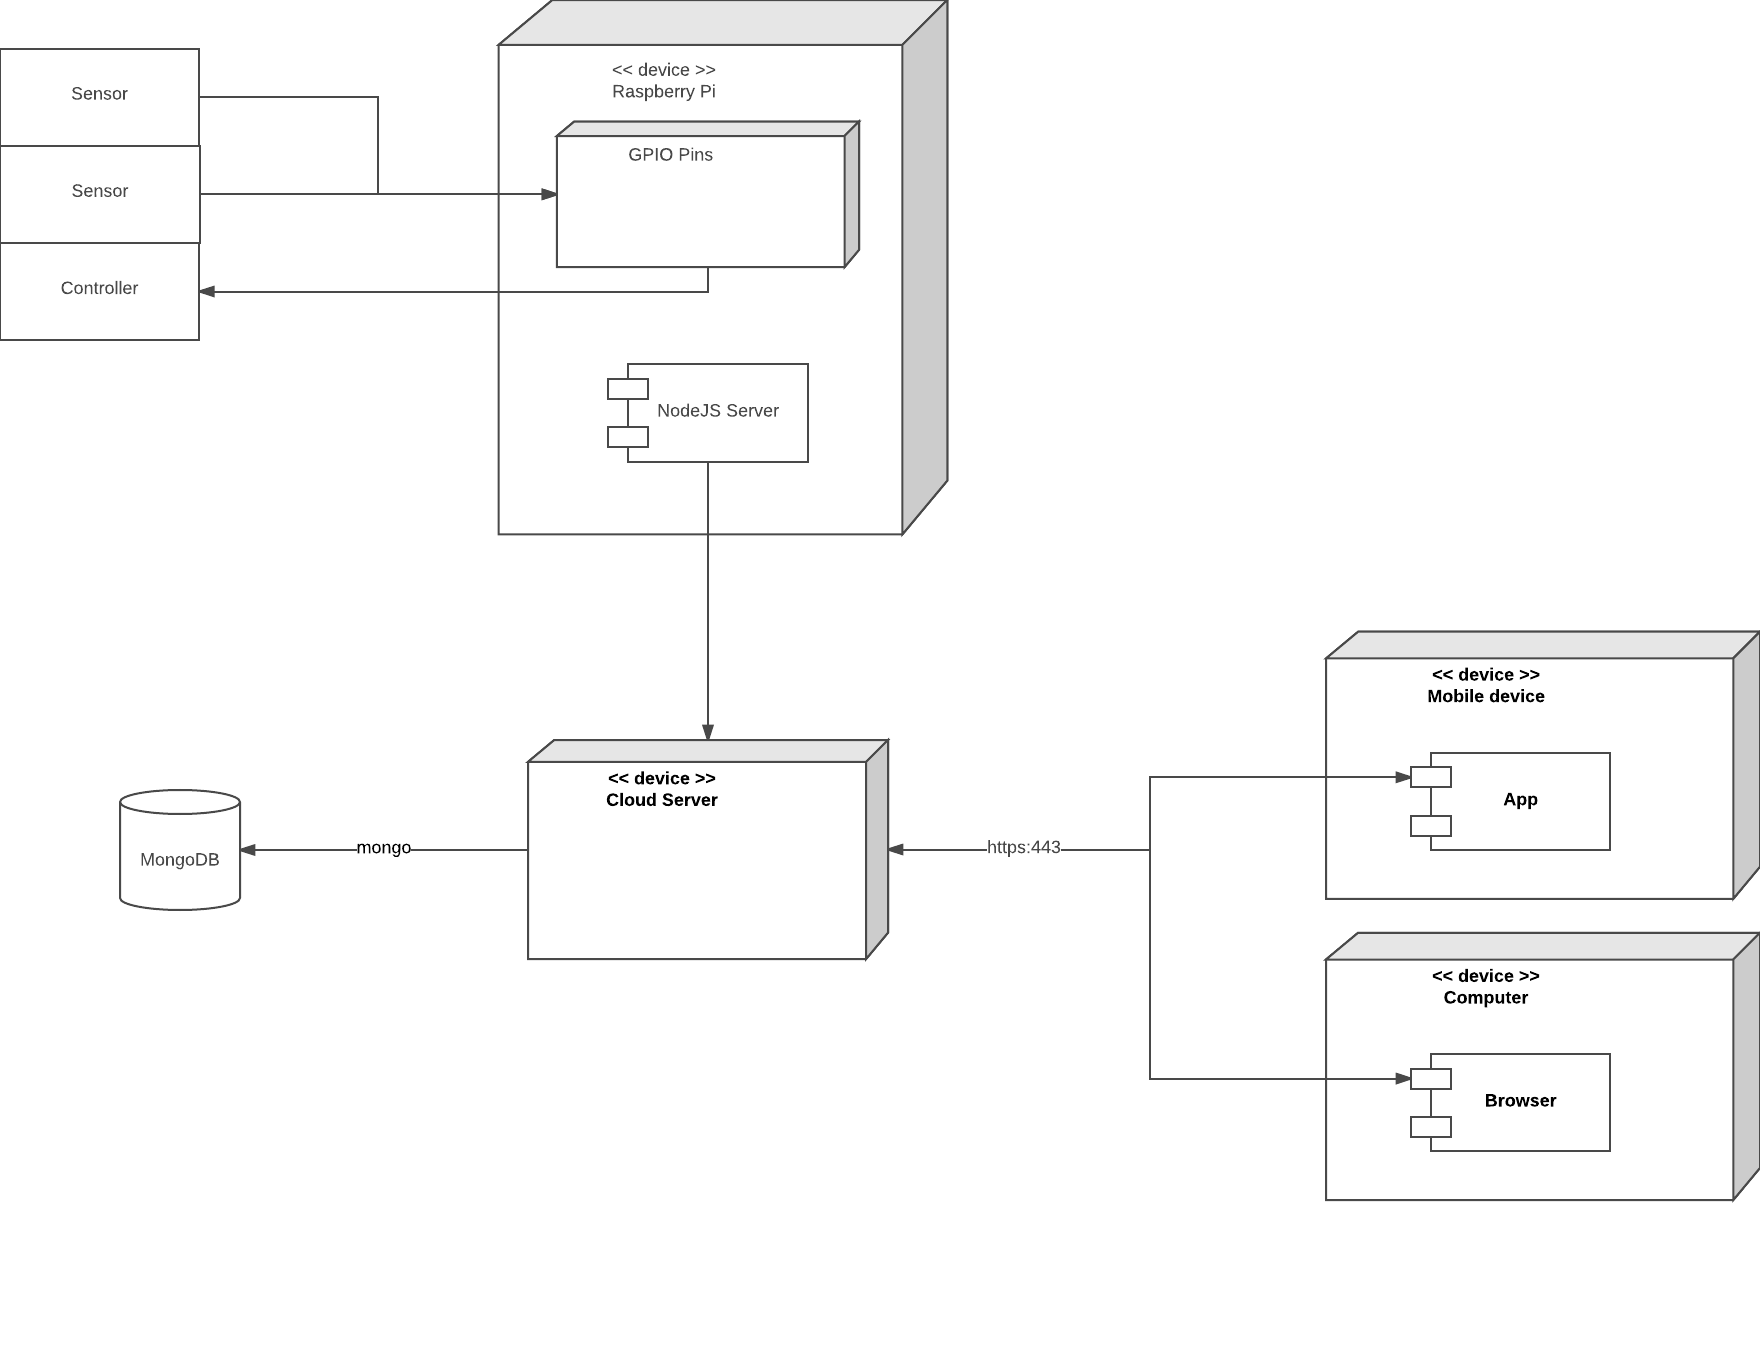
\includegraphics[width=0.8\textwidth]{deployment.png}}
	\caption{Deployment Diagram}
	\end{figure}
	\vfill
	\section{Proposed Methodology}
	 Praesent vel eros et metus imperdiet elementum eget gravida urna. Duis turpis diam, tempor vitae enim vitae, fermentum congue elit. Duis vitae scelerisque metus, et laoreet turpis. Nulla malesuada ligula ut suscipit vestibulum. In at iaculis urna. Mauris et dapibus nulla, ut auctor arcu. In consequat mollis sem sit amet viverra. Duis ante nulla, rutrum et mollis sed, condimentum at neque. Donec in leo eget massa gravida vestibulum. Praesent consequat turpis et tellus porta placerat. Ut mattis tempus tempor. Nullam vel elit vel nibh convallis consequat. Mauris consequat eros elit, ut maximus odio feugiat et. Praesent sed consectetur arcu.

In hac habitasse platea dictumst. Sed dictum vulputate molestie. Fusce placerat justo sed sem ullamcorper, a dictum ante mollis. Ut nisi augue, rutrum sit amet odio eget, ultricies maximus ex. Fusce finibus et metus sed elementum. Aenean at lacus nec nunc dignissim fringilla. Pellentesque placerat interdum iaculis. Curabitur finibus elit ac tincidunt aliquam. 
	\newpage
	\section{The Team}
	\textbf{Dimpho Mahoko} \\
	I am an aspiring software developer looking to gain new skills and develop those I already have. Notable skills include web development, Java, C++, JavaScript, PHP, HTML  \\ \\ %Should I list ALLLLLLLLLL My Skils????? I mean like ALLLLLLLLLL of them?????? Because I don't think we have enough time. Jokes. Seriously though. ALL the languages seems a bit tedious and also saying javascript does'nt imply node, angular and so on so should I add those too.  \\
	 Below are my accomplishments worth mentioning in no particular order.
	\begin{itemize}
		\item Second place in the Standard Bank IT challenge finals in 2016.\\
	
		\item Webmaster at Tuks FM from September 2016 till present. \\ 
			Responsibilities include maintaining the website and keeping it up to date. \\
			
		\item Mentor at The University of Pretoria EBIT Week for EBIT Marketing \\
			Responsibilities include database administration, website maintenance and all other admin related responsibilities like communication with parents whose children wish to attend EBIT Week. \\
			
		\item 2016 Retro Rabbit Rabbiteer program attendee \\
			The program was focused mainly on giving programming students an idea of how work in the industry is actually done. Notable technologies learnt include GitHub integration with team work and cloud computing and hosting. \\%I'll elaborate further
	\end{itemize}
	

\textbf{Jason van Hattum}\\ 
    I am a motivated developer with a passion for application and web-app development. Technologies that I am fluent in include full-stack MEAN and LAMP development, Java, C++, Android, Python and Django. I have experience in project management, web-app development and Android application development. \\
    
    I enjoy experimenting in my free time, especially working on side projects on my Raspberry Pi and building Android applications. I also enjoy making graphical programs in WebGL. My hobbies also include reading, playing games, and fishing. \\
    
    \noindent
    Projects that I have worked on include:
    \begin{itemize}
        \item A web application for the University of Pretoria used for peer-review and team evaluation within major projects (Can be found \href{https://github.com/teampinocchio/pinocchio/wiki}{\underline{here}}.). Skills that I developed here include front-end languages such as HTML, CSS, and Javascript; Python and Django.
    
        \item A variety of Android applications as a freelancing developer, both front-end and back-end. Skills developed here include Android development, Google Firebase, interface design and NodeJS.
    \end{itemize}
    
    \noindent
	Accomplishments and work experience:
    \begin{itemize}
        \item A member of the Golden Key International Honors Society.
        \item A teaching assistant and tutor for multiple subjects since January 2016.
        \item Participated in the Standard Bank IT Challenge in 2016 and 2017; and ACM in 2016.
        % \item Passed AI
        % \item Got destroyed in the Digital Gaming League, Dota division.
    \end{itemize}

\textbf{Kyle Erwin}\\
	Currently studying a BSc Computer science. I'm a well rounded programmer with many skills in many languages. My passion lies in artificial intelligence and creating applications with an intuitive design. I'm a harder worker that is known to be ``on top of things`` by my peers. \\ 

	I've worked in many leader positions and understand the importance of synergy in a team. Most noteworthy, I was apart of the TukVillage residence committee and the graphic desiner for all of the events (2015 - 2016). I launched a web development company, \href{www.unhinged.co.za}{\underline{unhinged.co.za}}, with team member Keagan Ferrett. My work has also extended to app development and partnerships with small startup companies.\\

	In my free time I often find myself programming on personal projects, coming up with new concepts and focusing my time on perfection my artificial intelligence skills. 

	\noindent
	More about me and my skills:
    \begin{itemize}
        \item Up-to-date with all the latest design trends.
        \item Used applications such as google analytics, webmaster and google trends. 
        \item Written many C++ tutorials for beginner programmers
        \item Business skills and working with clients. 
        \item An understanding of scala, a programming language great for AI. 
    \end{itemize}

    \end{itemize}
\textbf{Joshua Cilliers}\\
Lorem ipsum dolor sit amet, consectetur adipiscing elit. Curabitur aliquam augue a odio cursus bibendum. Suspendisse felis diam, varius eu molestie quis, condimentum eget libero. Fusce egestas ligula sit amet metus vehicula ornare. Integer et magna sapien. Pellentesque nec metus in sapien congue gravida eu quis dolor. Maecenas consequat nunc a enim ullamcorper venenatis. Suspendisse at faucibus dolor, imperdiet rhoncus ante. \\ \\
\textbf{Keegan Ferrett}\\
Lorem ipsum dolor sit amet, consectetur adipiscing elit. Curabitur aliquam augue a odio cursus bibendum. Suspendisse felis diam, varius eu molestie quis, condimentum eget libero. Fusce egestas ligula sit amet metus vehicula ornare. Integer et magna sapien. Pellentesque nec metus in sapien congue gravida eu quis dolor. Maecenas consequat nunc a enim ullamcorper venenatis. Suspendisse at faucibus dolor, imperdiet rhoncus ante.

\end{document}

	\newpage
	\section{Why Albert Prime?}
	\begin{center}
    	
\includegraphics[width=4cm]{../Common/AlbertPrimeLogo.png}
	\end{center}
	Our team consists of a set of people with enough skills to complete this project sufficiently and then some. We are all sufficiently competent in MEAN stack. \\ 
	
	Keegan is our resident Raspberry Pi expert. He has a passion for Raspberry Pi and works with them on a regular basis. This will aid the development of this system as one of the requirements is to program a Raspberry Pi to gather the data from the devices around the house.\\
	
	As third year Computer Science Students, we know a number of programming languages. It is worth mentioning that Jason is very fluent in Python amongst other languages. It will be an asset to your system to have someone with his expertise working on it.\\
	
	
	Application development is one of our strong points. The mobile application needed for the caretaker communication and control of devices will make use of our skills. Joshua and Keegan's experience with iOS and Android development and his passion for mobile application development amongst others will be put to great use with this system.\\
	
	This system will require creativity and and a good understanding of cloud servers. The Rabbiteer program Dimpho attended in 2016 focused a lot on this. This project will be an opportunity to develop these skills and her success in the Standard bank IT challenge shows her creative capability and competence.\\
	
	Kyle is very passionate about Artificial Intelligence which is always a useful skill in today's age. This system could use his passion and skill for the monitoring and learning the user's patterns such that if anything seems out of place, the caregivers can notified.\\
	
	All 5 group members are talented developers. Above are a few of the skills we have to offer but our skills are not limited to what is mentioned above. We are all hardworking fast learners and willing to learn any new technologies and skills needed to make this system a successful one. \\
	\begin{figure}[htb]
	\centering
	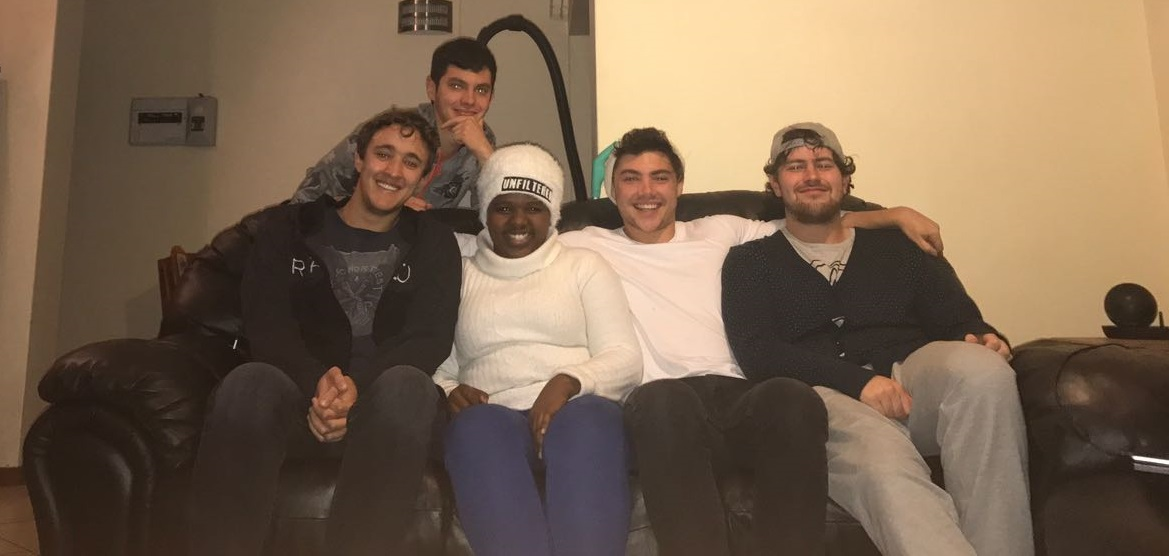
\includegraphics[width=\textwidth]{../Common/team.jpg}
	\caption{The Squad}
	\end{figure}\\
	
\end{document}